\subsubsection{February 2023}

Welcome to the February 2023 OpenScienceLab Update!

\subparagraph{Changes:}

\begin{itemize}
\item OpenScienceLab
\item Single~Sign~On
\item Automatic~Authentication
\item User~Access
\item IP~Filter
\item User~Request
\item Multi~Download
\item Kernel~Usage
\item Recommended~Jupyter~Notebook~Changes
\end{itemize}


\bigskip
\centerline{\rule{13cm}{0.4pt}}
\bigskip

\paragraph{\textbf{OpenScienceLab}}\label{opensciencelab}

\begin{itemize}
\item OpenSARLab is now a part of OpenScienceLab with significant changes. Users can access different courses from a single page.
\end{itemize}

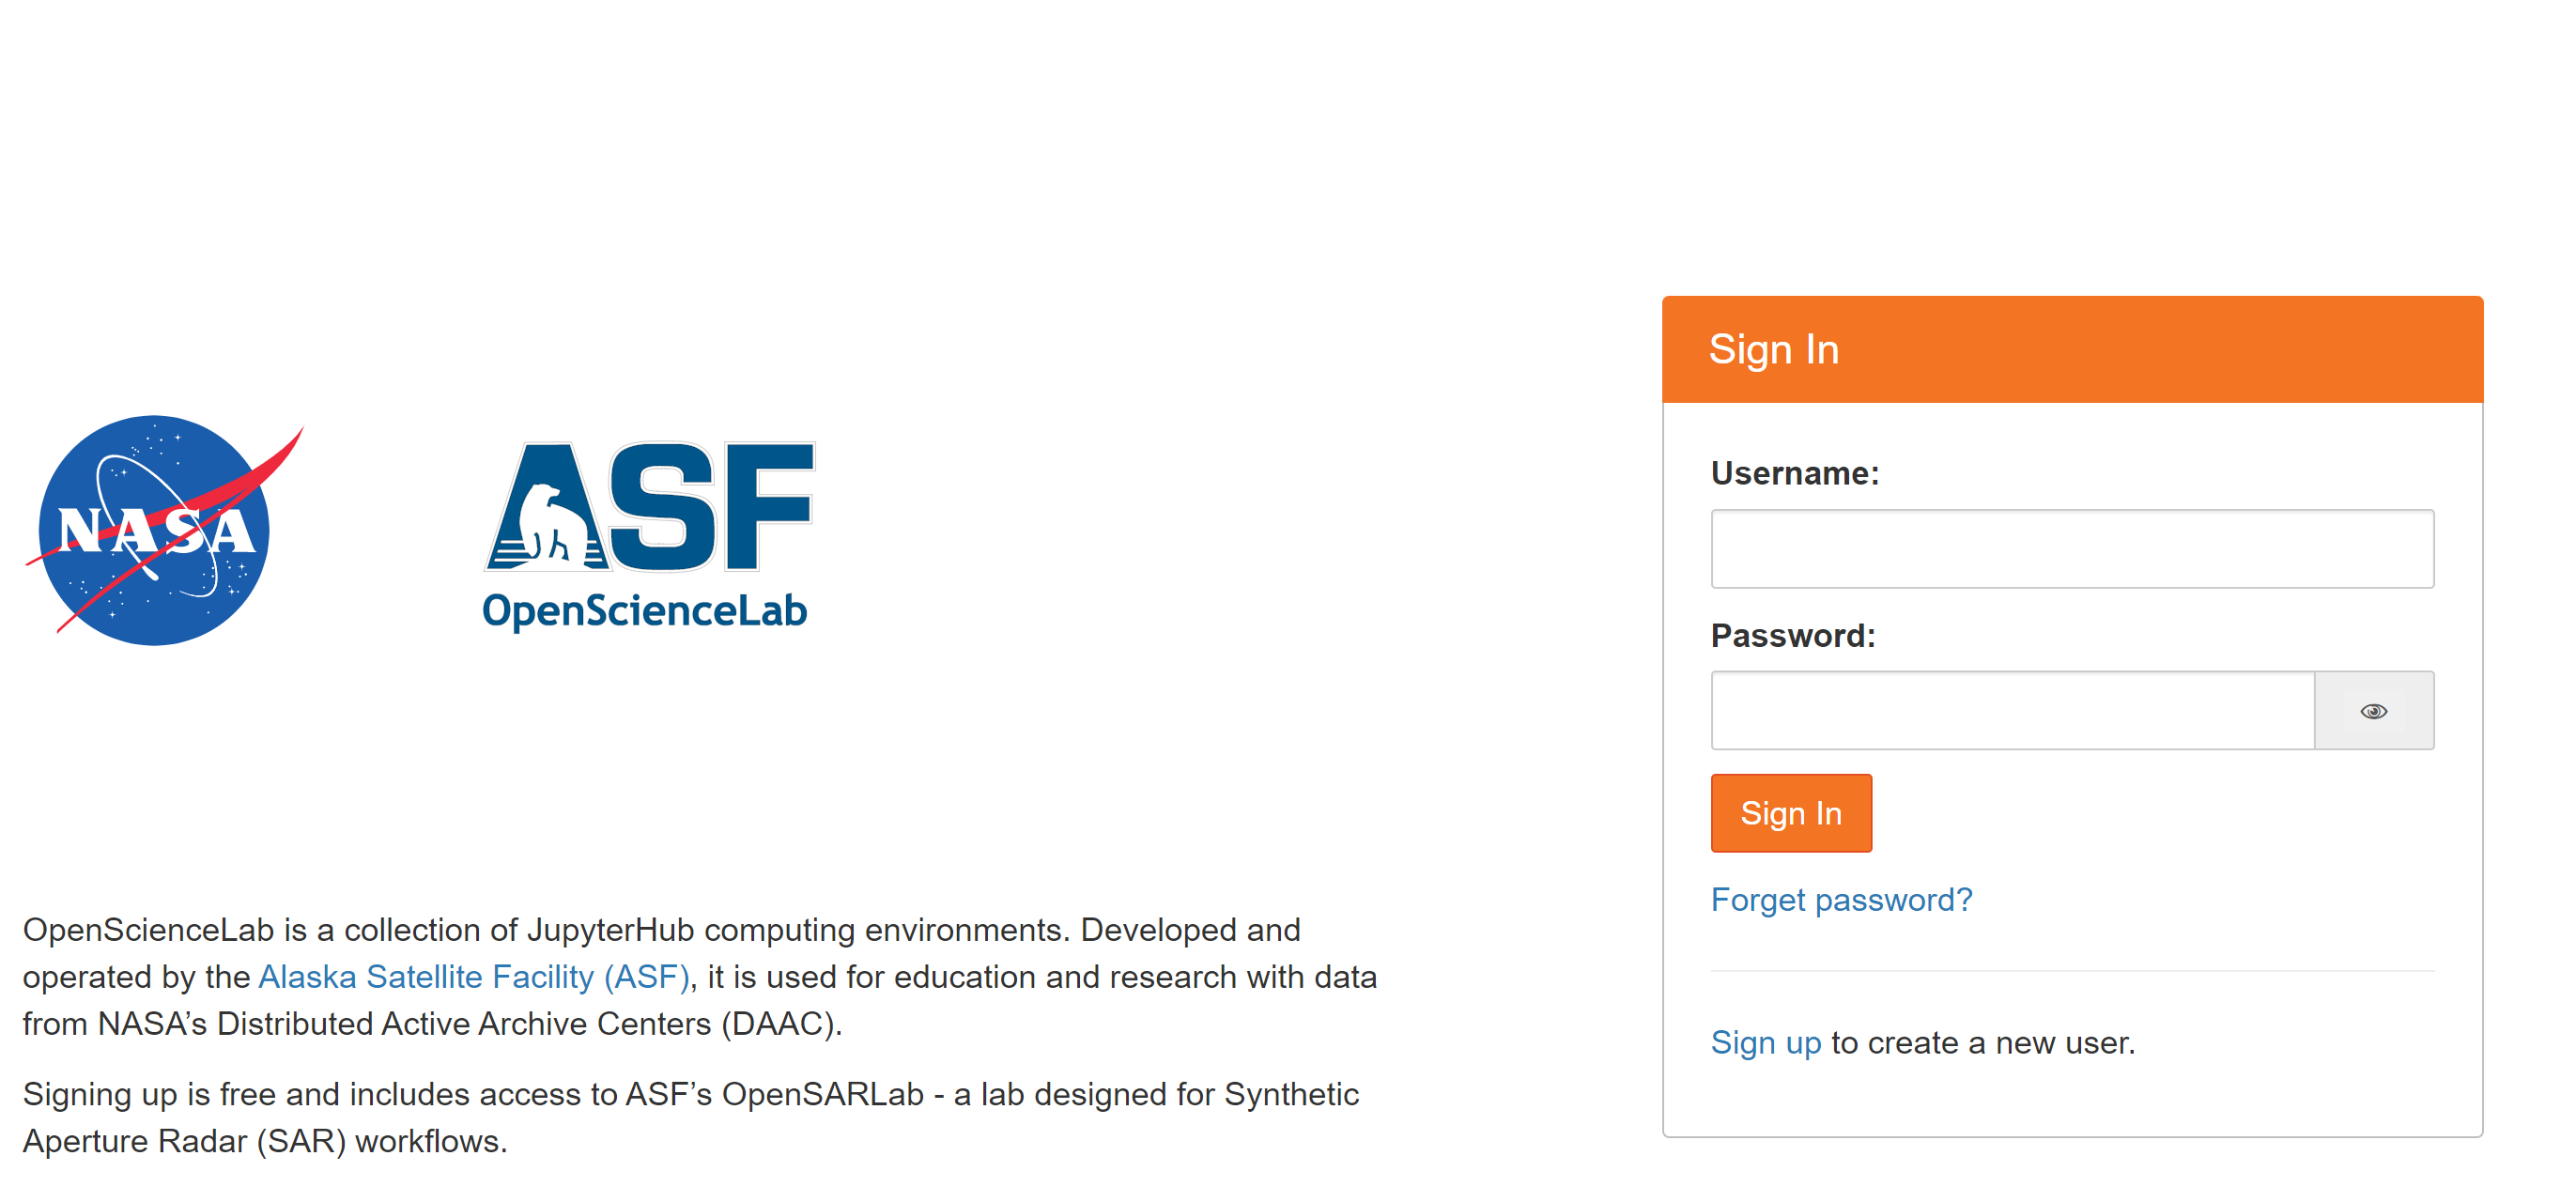
\includegraphics[width=0.7\linewidth]{files/opensciencelab-8e85c9cc58445dc01847745b03f7ec57.PNG}

\paragraph{\textbf{Single Sign On}}\label{single-sign-on}

\begin{itemize}
\item New single sign-on (SSO) to simplify the logging-in process. SSO eliminates the burden of the sign-on process by listing all accounts on a single web page with additional layers of security.
\end{itemize}

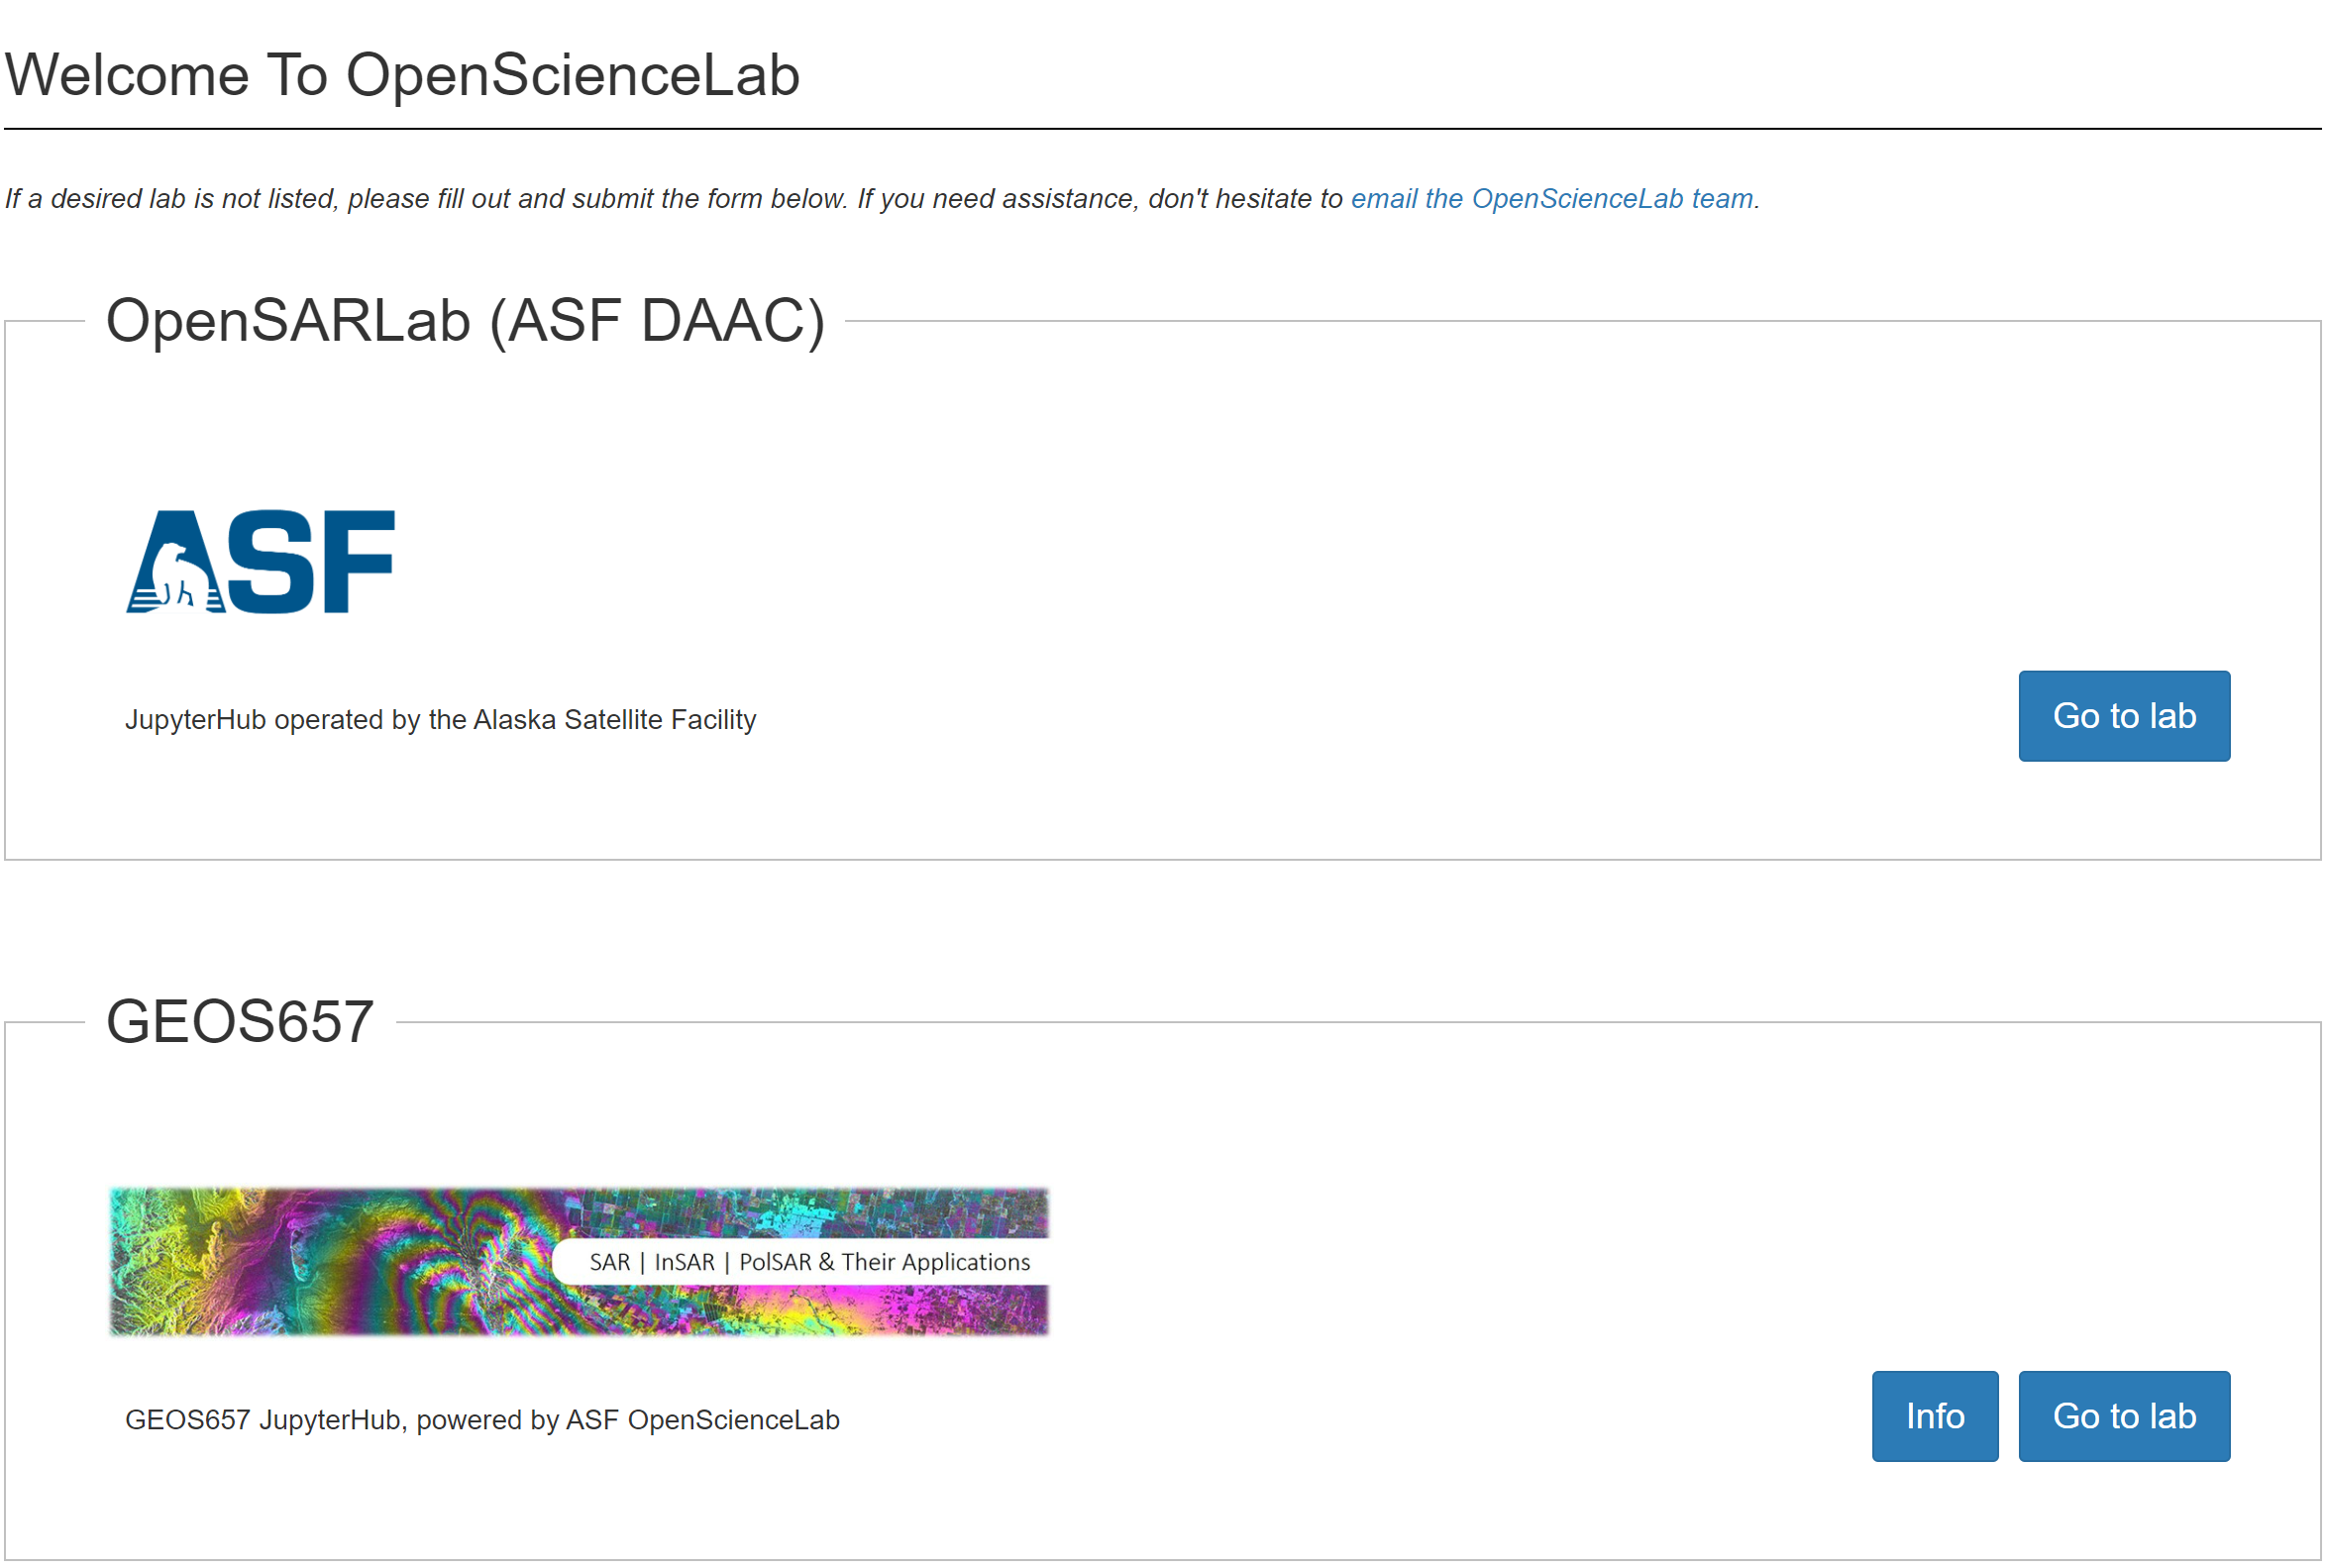
\includegraphics[width=0.7\linewidth]{files/single_sign_on-89eb0d255f0daa91c661c0a2359a6916.PNG}

\paragraph{\textbf{Automatic Authentication}}\label{automatic-authentication}

\begin{itemize}
\item Users who sign up to the OpenScienceLab no longer need admins to activate their accounts.
\end{itemize}

\paragraph{\textbf{User Access}}\label{user-access}

\begin{itemize}
\item Admins can easily give users access to different profiles from a single page. Admins can toggle access lists based on various deployments.
\end{itemize}

\paragraph{\textbf{IP Filter}}\label{ip-filter}

\begin{itemize}
\item OpenScienceLab will prevent users in one of NASA's \href{https://www.nasa.gov/sites/default/files/atoms/files/designated\_country\_list\_6.10.2022.pdf}{designated countries list} from creating an account so that we are compliant with NASA's security protocol.
\end{itemize}

\paragraph{\textbf{User Request}}\label{user-resquest}

\begin{itemize}
\item Users can send a request to the OpenScienceLab team from the portal.
\end{itemize}

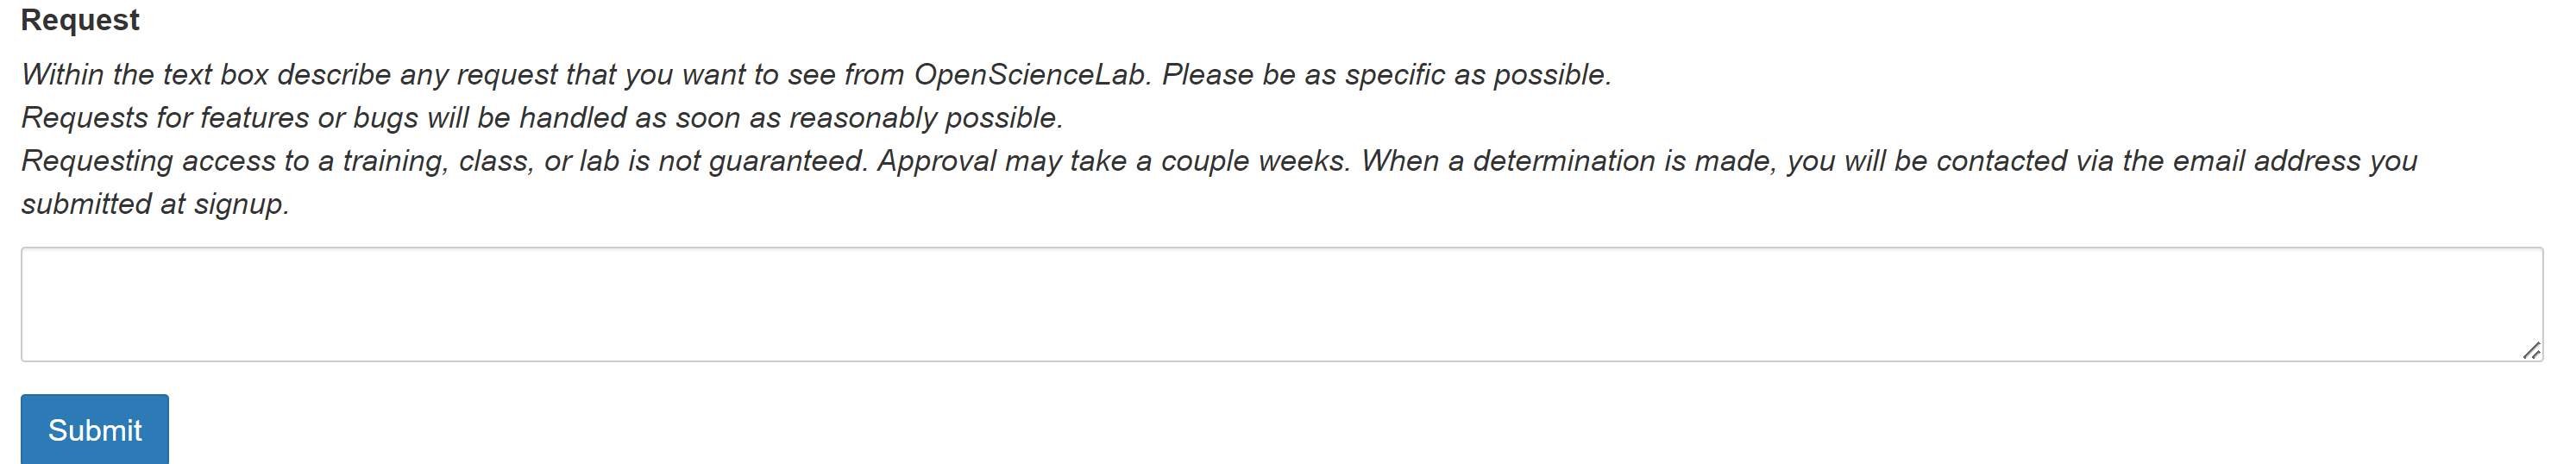
\includegraphics[width=0.7\linewidth]{files/user_request-b4d8f393b11dea7c2cbf0b3baf130dba.PNG}

\paragraph{\textbf{Multi Download}}\label{multi-download}

\begin{itemize}
\item Users can download multiple files at once through OpenScienceLab.
\item \textbf{NB}: Downloading multiple directories requires users to compress the directories beforehand.
\end{itemize}

\includegraphics[width=0.7\linewidth]{files/multi_download-5ee606c2f5273c98a62c6238687f7413.gif}

\paragraph{\textbf{Kernel Usage}}\label{kernel-usage}

\begin{itemize}
\item The latest update of JupyterLab has a built-in kernel monitor that tracks detailed resource usage, such as:\begin{itemize}
\item Kernel Host
\item Memory consumption and availability
\item CPU usage
\end{itemize}
\end{itemize}

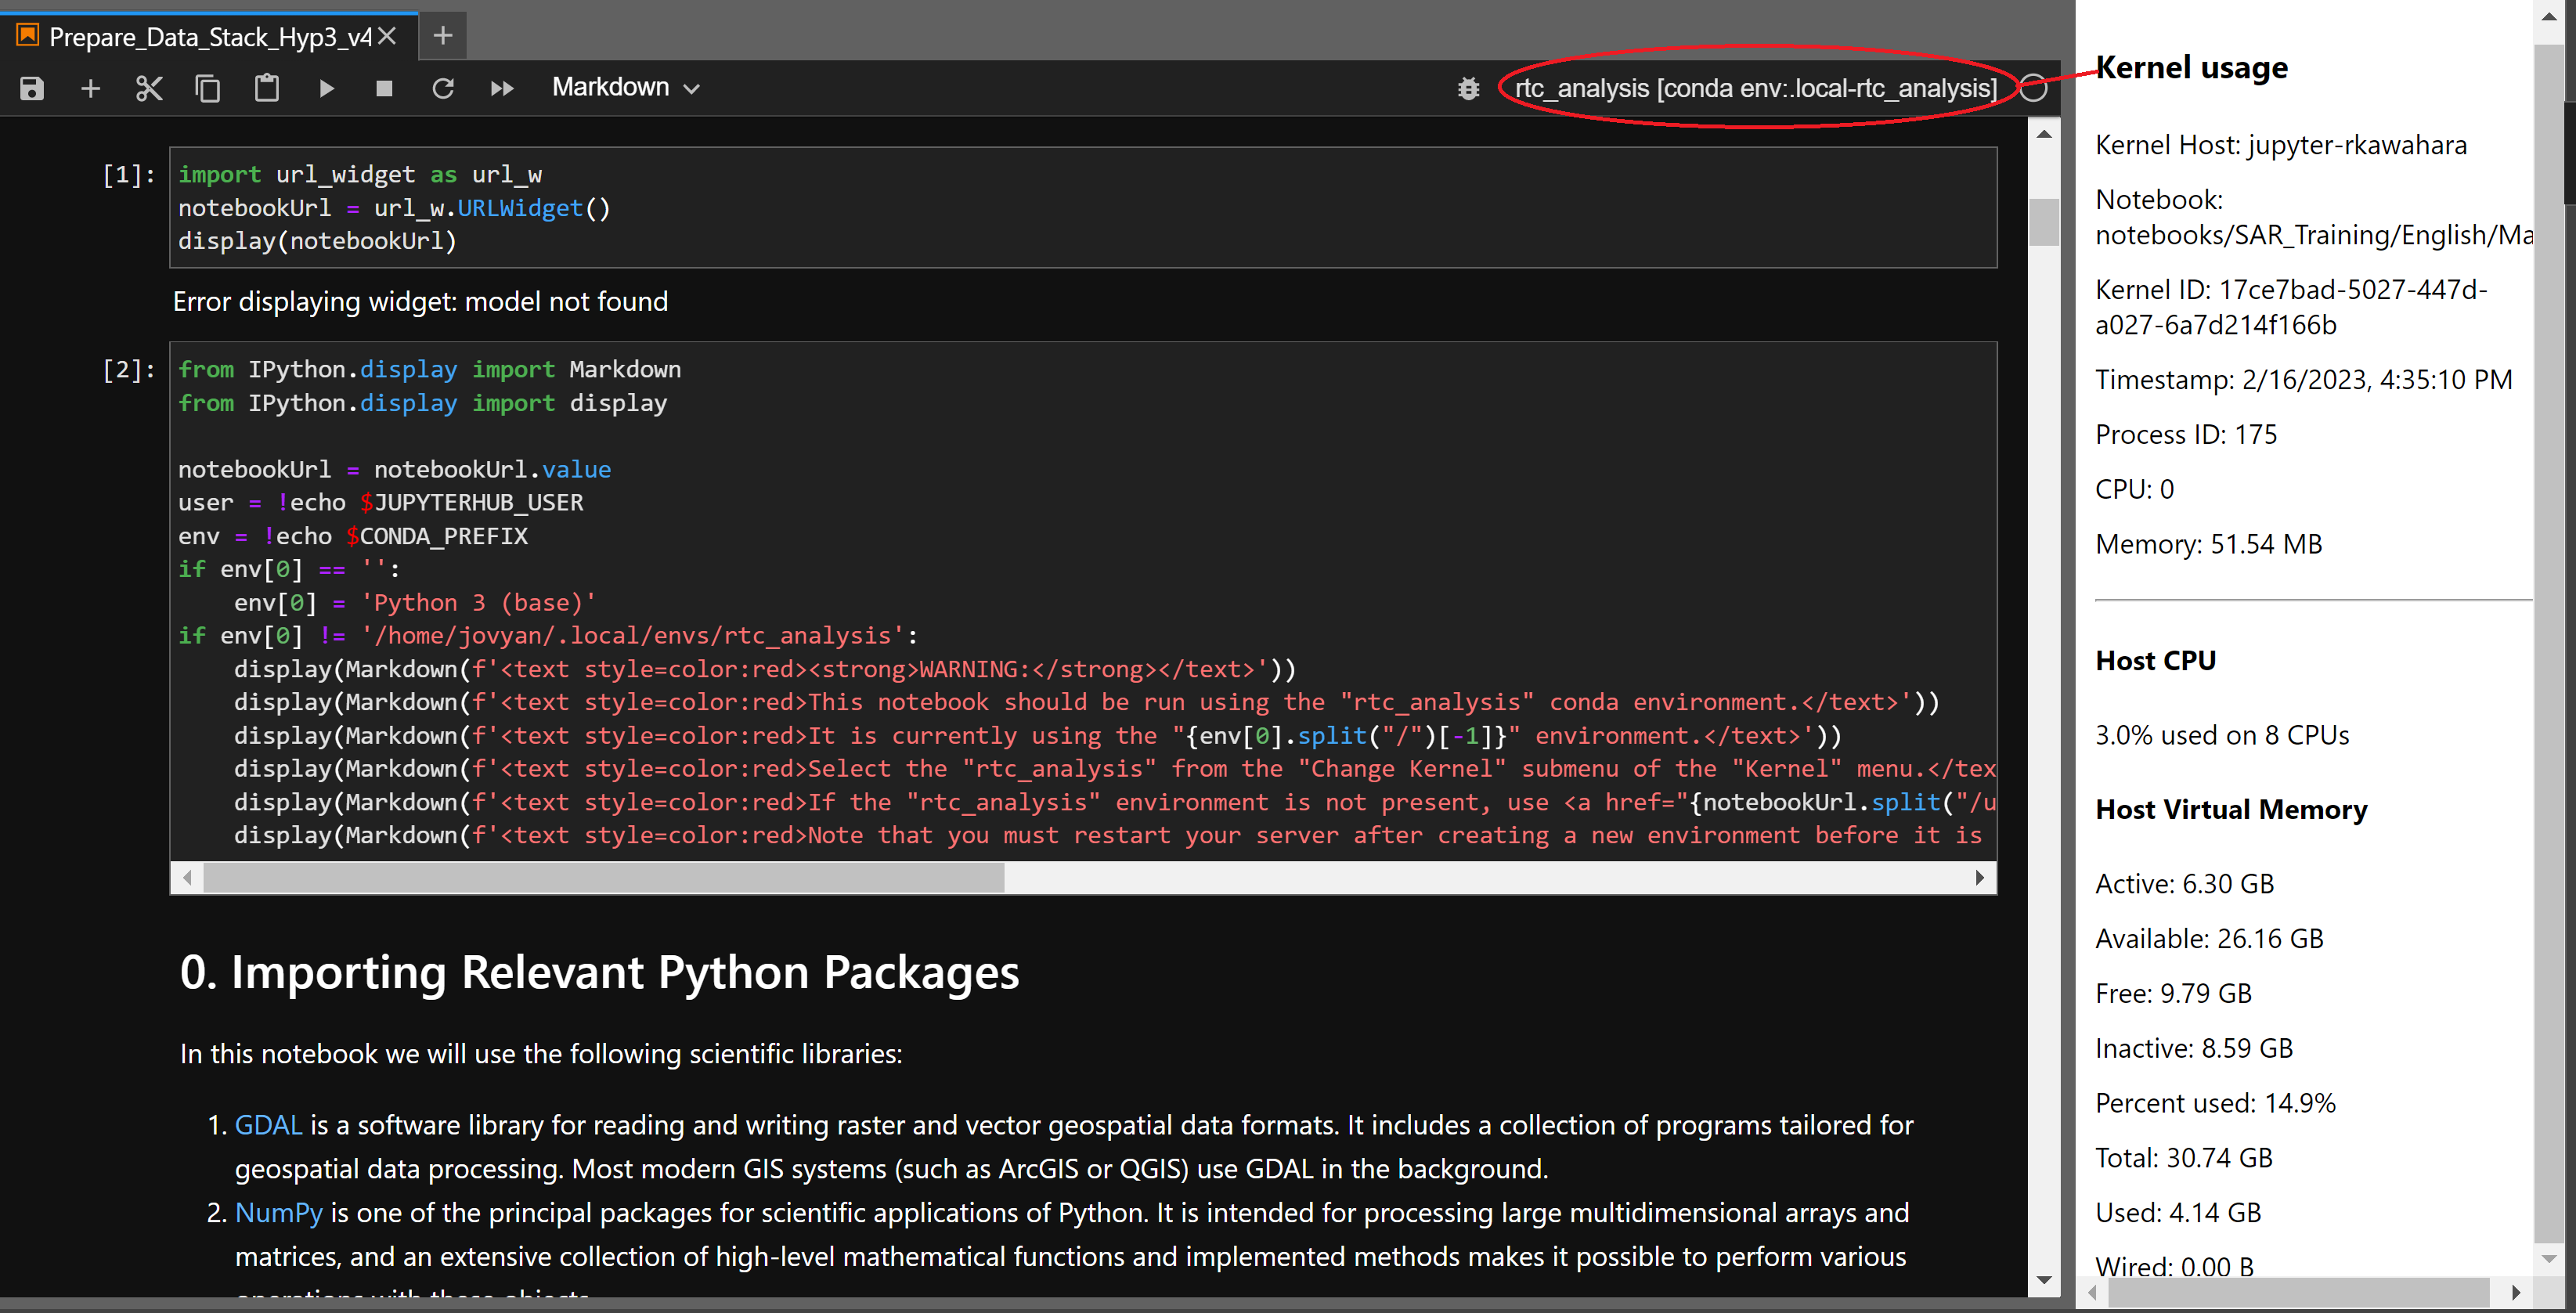
\includegraphics[width=0.7\linewidth]{files/kernel_usage-3999565cdea65e09da8c3bdf1ec55131.PNG}

\paragraph{\textbf{Recommended Jupyter Notebook Changes}}\label{recommended-jupyter-notebook-changes}

The following bullet points cover code changes you may need to make to your notebooks for them to work in JupyterLab:

\begin{itemize}
\item MintPy Update:

Due to the recent MintPy update, import syntax for version 1.4.1+ differs from previous versions. As a result, some notebooks may be incompatible with the latest version of MintPy. Below are examples of how to import MintPy depending on which versions you have:

\begin{verbatim}
# version 1.4.0 and below:
import mintpy.view as view
import mintpy.tsview as tsview
.
.
.

# version 1.4.1+
from mintpy.cli import view, tsview, ...
\end{verbatim}
\end{itemize}

For additional backward compatibility changes, please refer to the previous release notes.